\documentclass[convert={density=600,outext=.png},tikz,crop=true,border=3pt]{standalone}
\usetikzlibrary{arrows,shapes,positioning}
\usetikzlibrary{calc,decorations.markings}

\usepackage{tikz-qtree}
\usepackage{makecell}   % for multiline labels



\begin{document}


	% illustration of a tree
	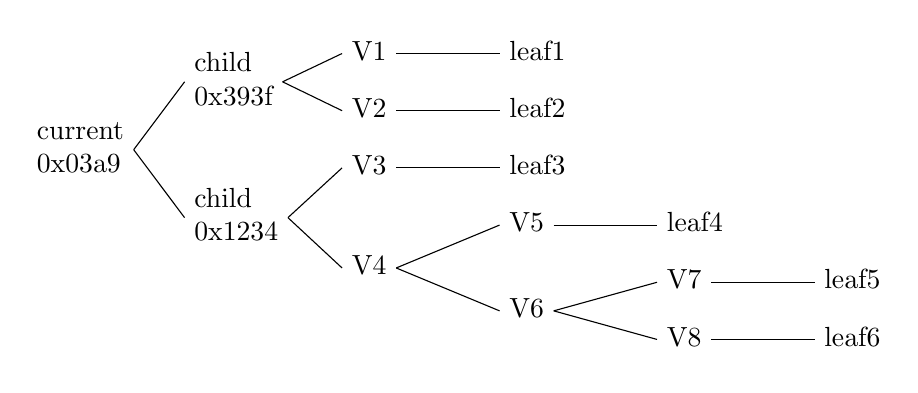
\begin{tikzpicture}
		\tikzset{grow'=right, level distance=2cm}
		\tikzset{execute at begin node=\strut}
		\tikzset{every tree node/.style={anchor=base west}}


		\Tree [.{\makecell[l]{current \\ 0x03a9}}
				[.\makecell[l]{child \\ 0x393f} [.V1 leaf1 ] [.V2 leaf2 ] ]
				[.\makecell[l]{child \\ 0x1234} [.V3 leaf3 ]
							[.V4 	[.V5 leaf4 ]
								[.V6 	[.V7 leaf5 ]
									[.V8 leaf6 ] ] ] ] ]
	\end{tikzpicture}
	


\end{document}